\documentclass[10pt,a4paper]{article}
\usepackage[utf8]{inputenc}
\usepackage[german]{babel}
\usepackage[T1]{fontenc}
\usepackage{amsmath}
\usepackage{amsfonts}
\usepackage{amssymb}
\usepackage{float}
\usepackage{graphicx}
\usepackage{listings}
\renewcommand\thesubsection{\alph{subsection}}
\begin{document}

\begin{center}
Modellierung hybrider Systeme mit Stateflow: Praktikum 3

Johannes Reidl, Sigurd Sippel

\end{center}

\section{Start einer zweistufigen Rakete}

	\begin{figure}[H]
 	 		\centering
 	 		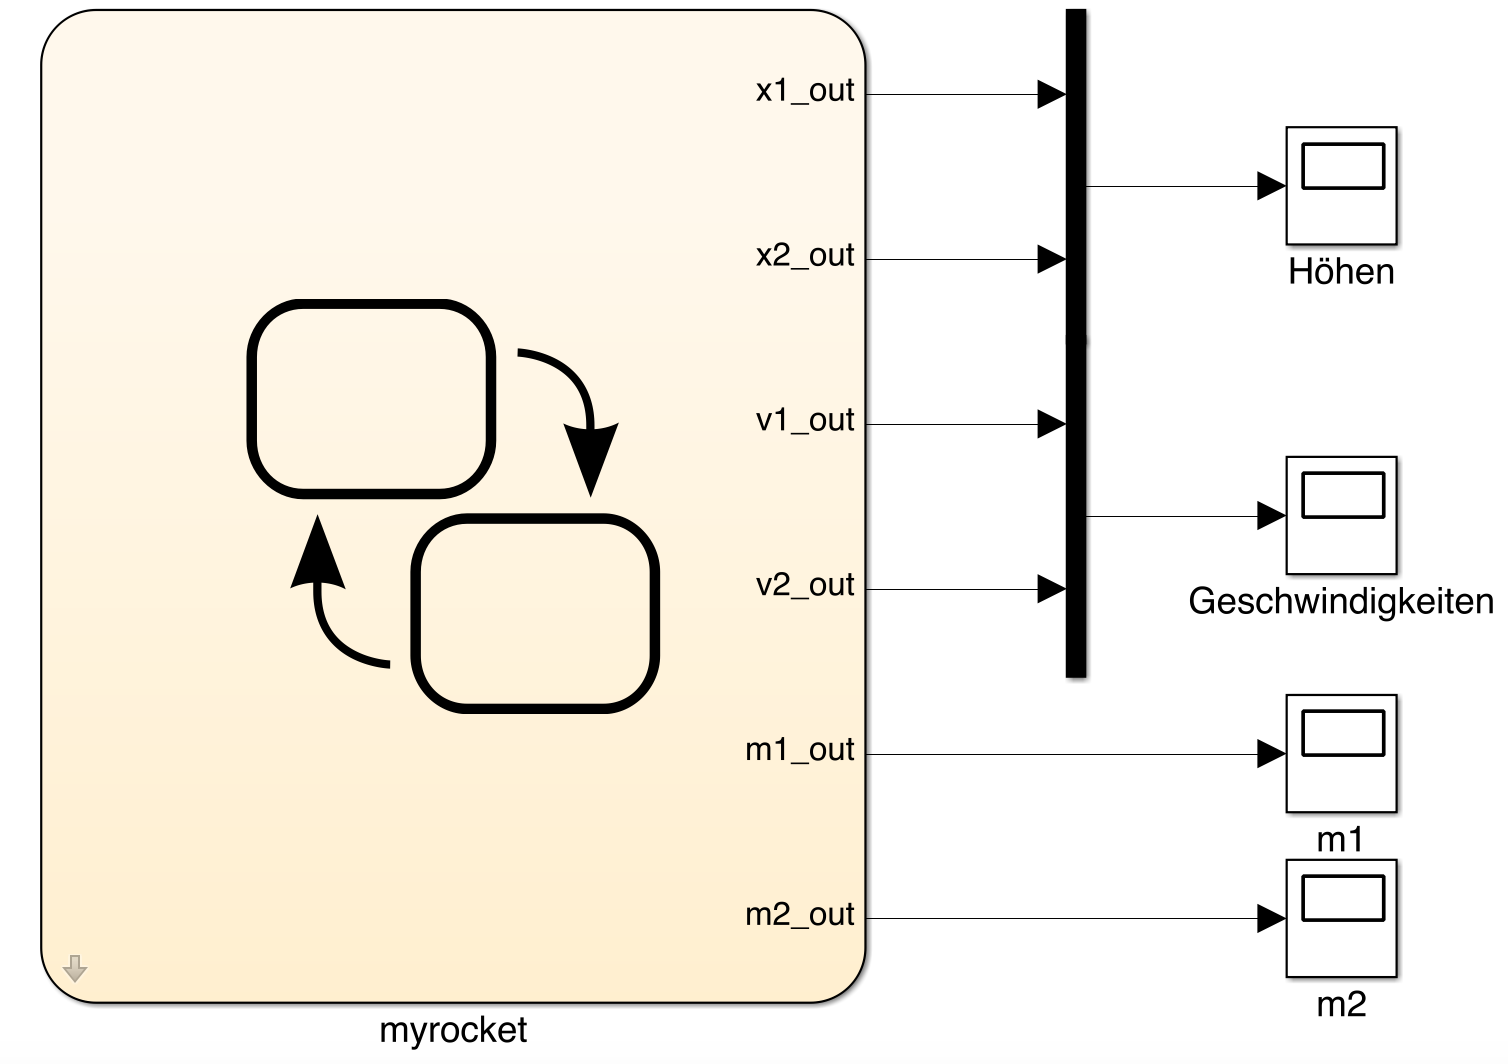
\includegraphics[width=1\textwidth]{../aufgabe1/screens/rocket_outer.png}
 	 		\caption{Simulink Stateflow}
 	 	\end{figure}

	\begin{figure}[H]
 	 		\centering
 	 		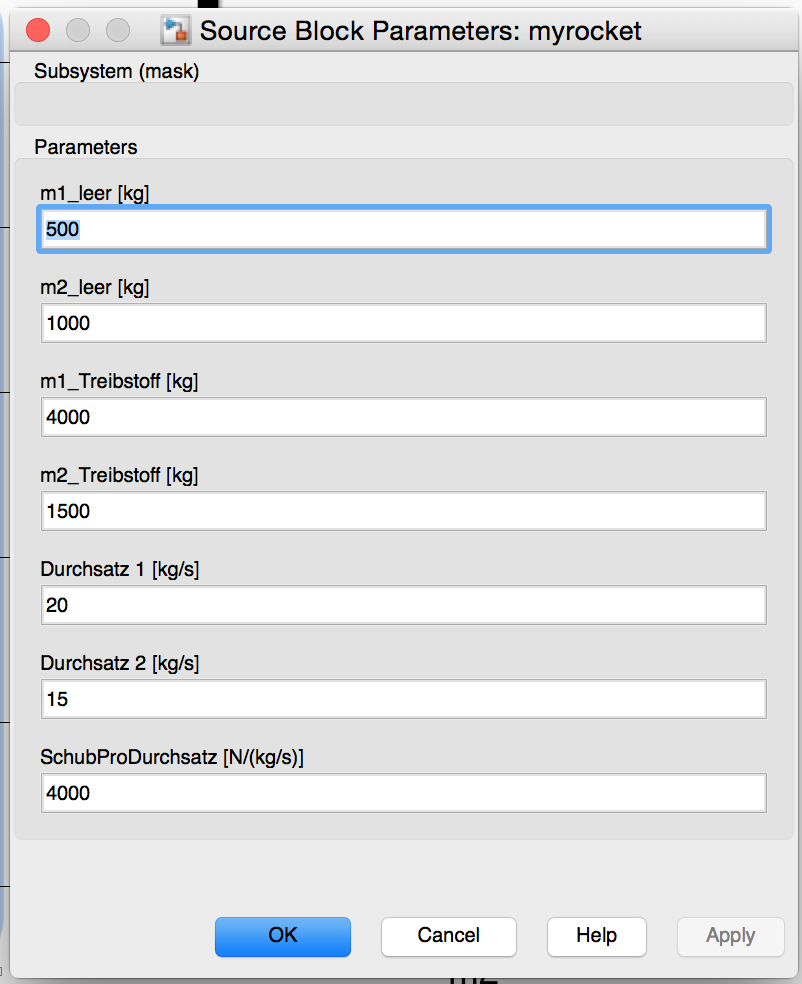
\includegraphics[width=1\textwidth]{../aufgabe1/screens/rocket_para.png}
 	 		\caption{Simulink Stateflow}
 	 	\end{figure}

		\begin{figure}[H]
 	 		\centering
 	 		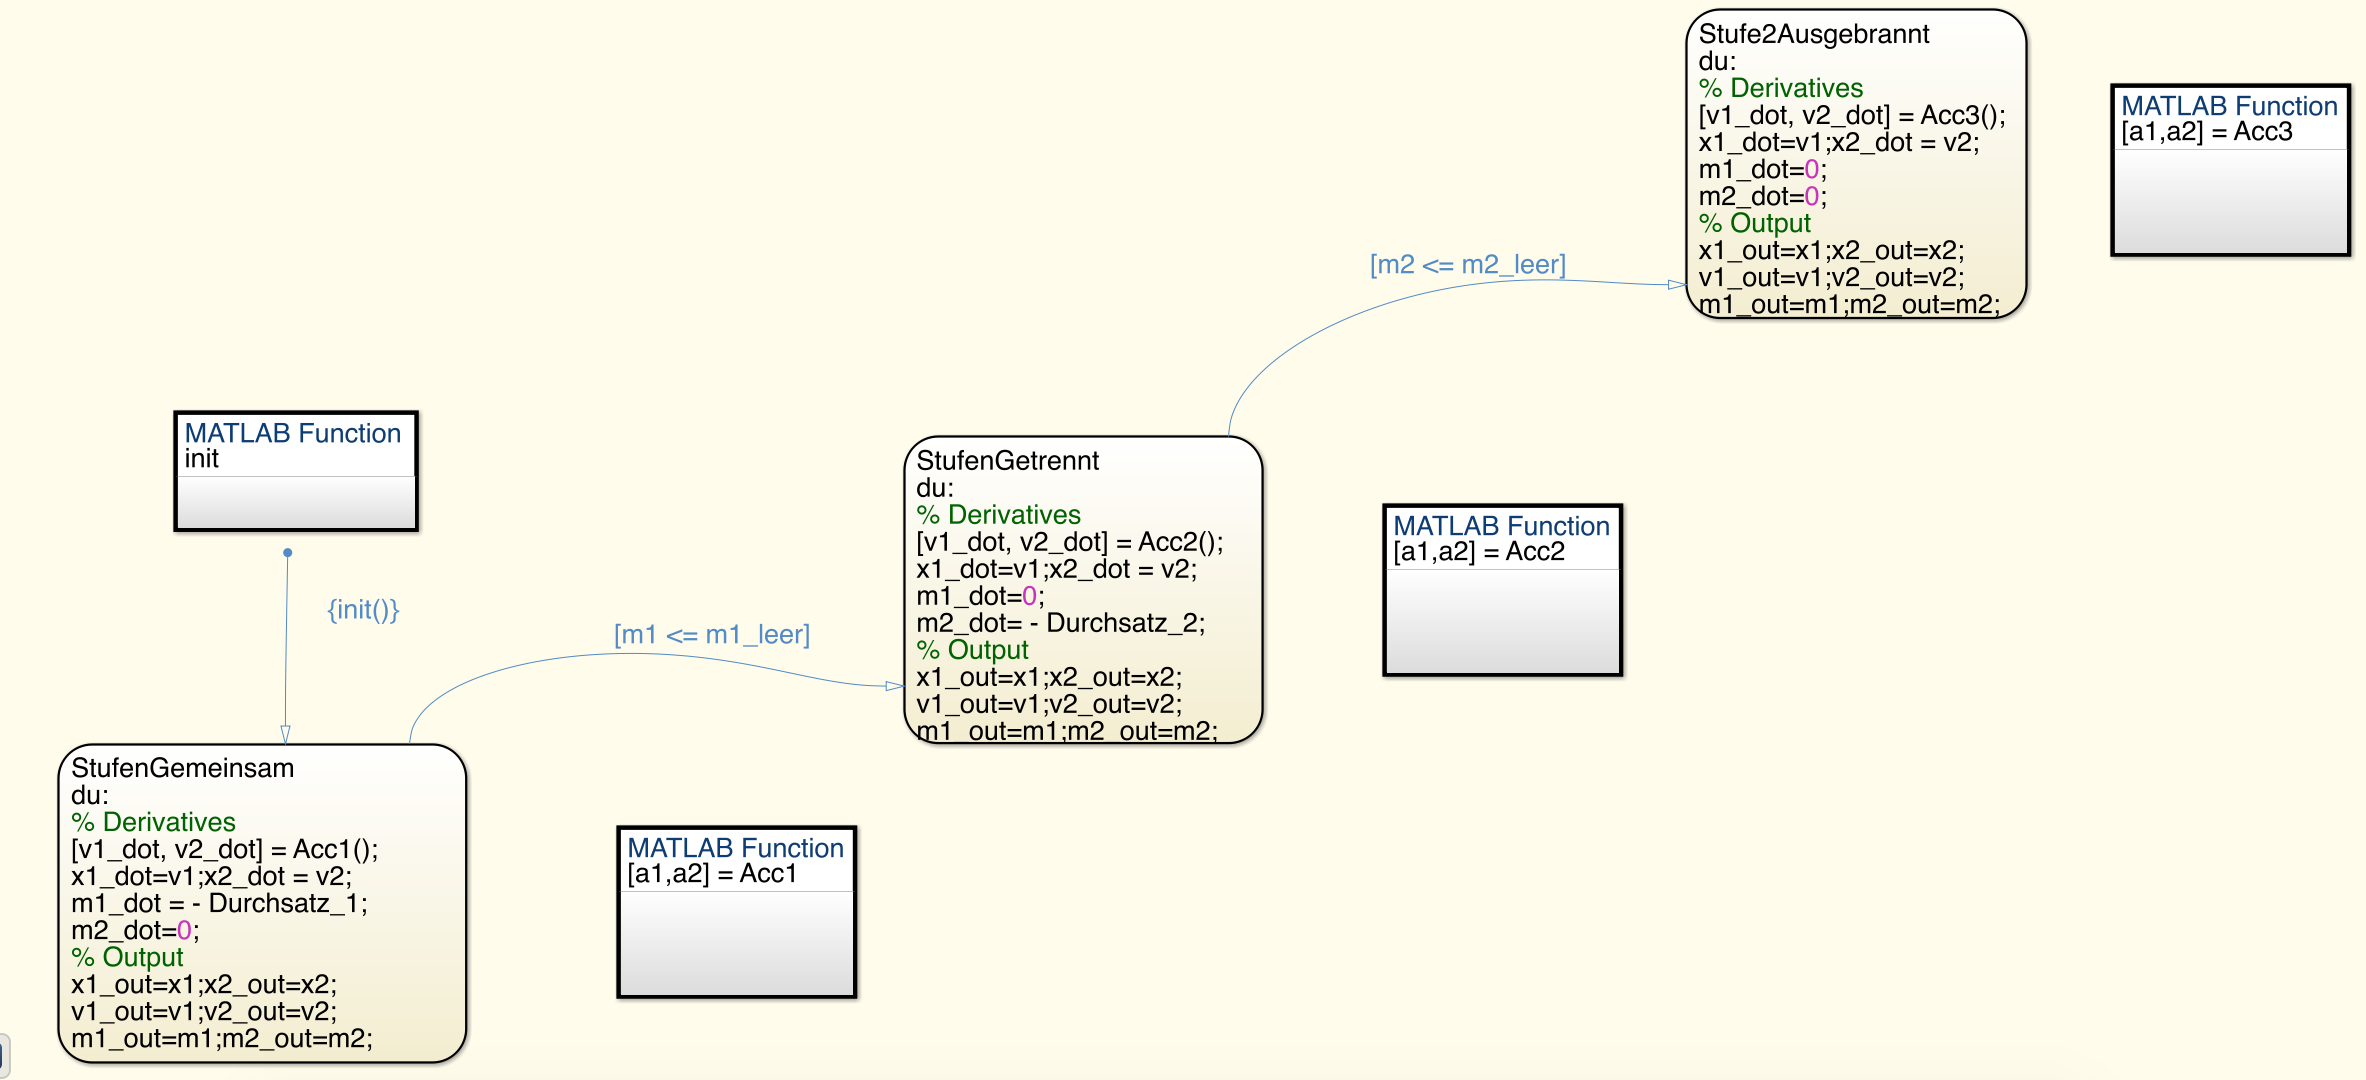
\includegraphics[width=1\textwidth]{../aufgabe1/screens/rocket_state.png}
 	 		\caption{Simulink States}
 	 	\end{figure}
 	 	
 	 	\begin{align}
 	 	Acc1 = 
 	 	\\mR = m1 + m2 \nonumber
 	 	\\r1 = x1 + rE \nonumber
 	 	\\Fs1 = G * (mE * mR) / (r1*r1) \nonumber
 	 	\\Schubkraft_1 = Durchsatz_1 * SchubProDurchsatz \nonumber
 	 	\\a = (Schubkraft_1 - Fs1) / (m1+m2) \nonumber
 	 	\\a1 = a \nonumber
 	 	\\a2 = a \nonumber
 	 	\end{align}
 	 	
 	 	\begin{align}
 	 	Acc2 =	 	 
 	 	\\r1 = x1 + rE \nonumber
 	 	\\Fs1 = G * (mE * m1) / (r1*r1) \nonumber
 	 	\\r2 = x2 + rE \nonumber
 	 	\\Fs2 = G * (mE * m2) / (r2*r2) \nonumber
 	 	\\Schubkraft_2 = Durchsatz_2 * SchubProDurchsatz \nonumber
 	 	\\a1 = - Fs1 / m1 \nonumber
 	 	\\a2 = (Schubkraft_2- Fs2) / m2 \nonumber
 	 	\end{align}

\begin{align}
Acc3 =
\\r1 = x1 + rE \nonumber
\\Fs1 = G * (mE * m1) / (r1*r1) \nonumber
\\r2 = x2 + rE \nonumber
\\Fs2 = G * (mE * m2) / (r2*r2) \nonumber
\\a1 = - Fs1 / m1 \nonumber
\\a2 = - Fs2 / m2 \nonumber
\end{align}

		 		\begin{figure}[H]
	 	 	 	 		\centering
	 	 	 	 		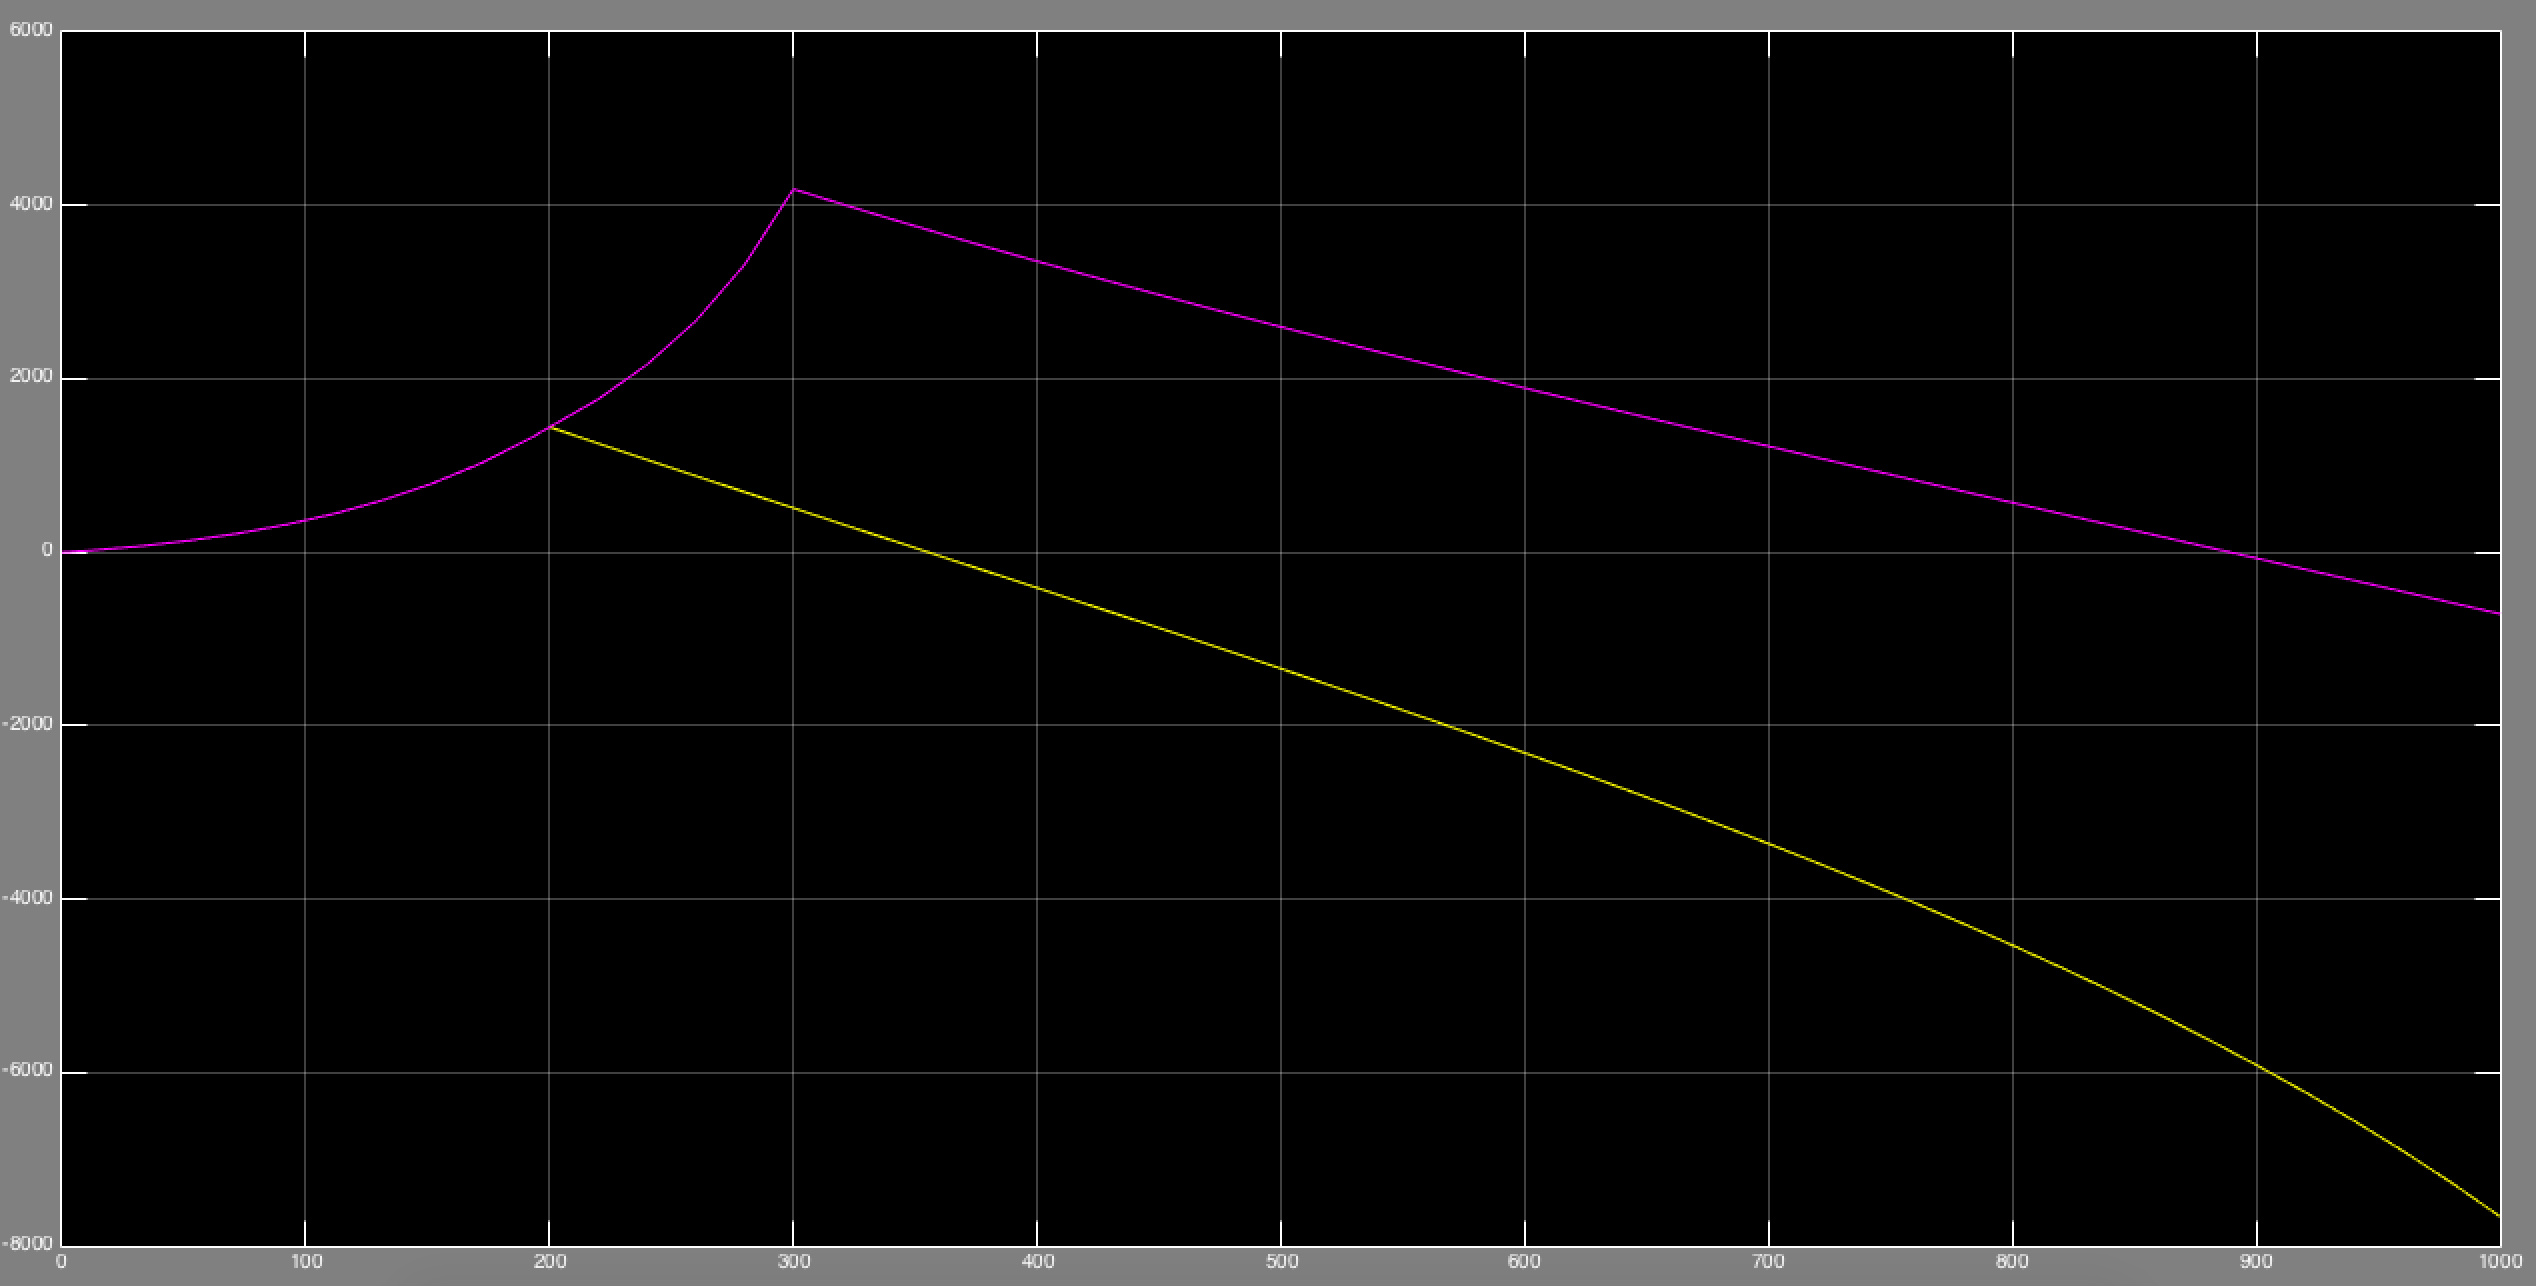
\includegraphics[width=1\textwidth]{../aufgabe1/screens/geschwindigkeiten.png}
	 	 	 	 		\caption{Geschwindigkeiten}
	 	 	 	 	\end{figure}
		 		\begin{figure}[H]
		 	 	 	 		\centering
		 	 	 	 		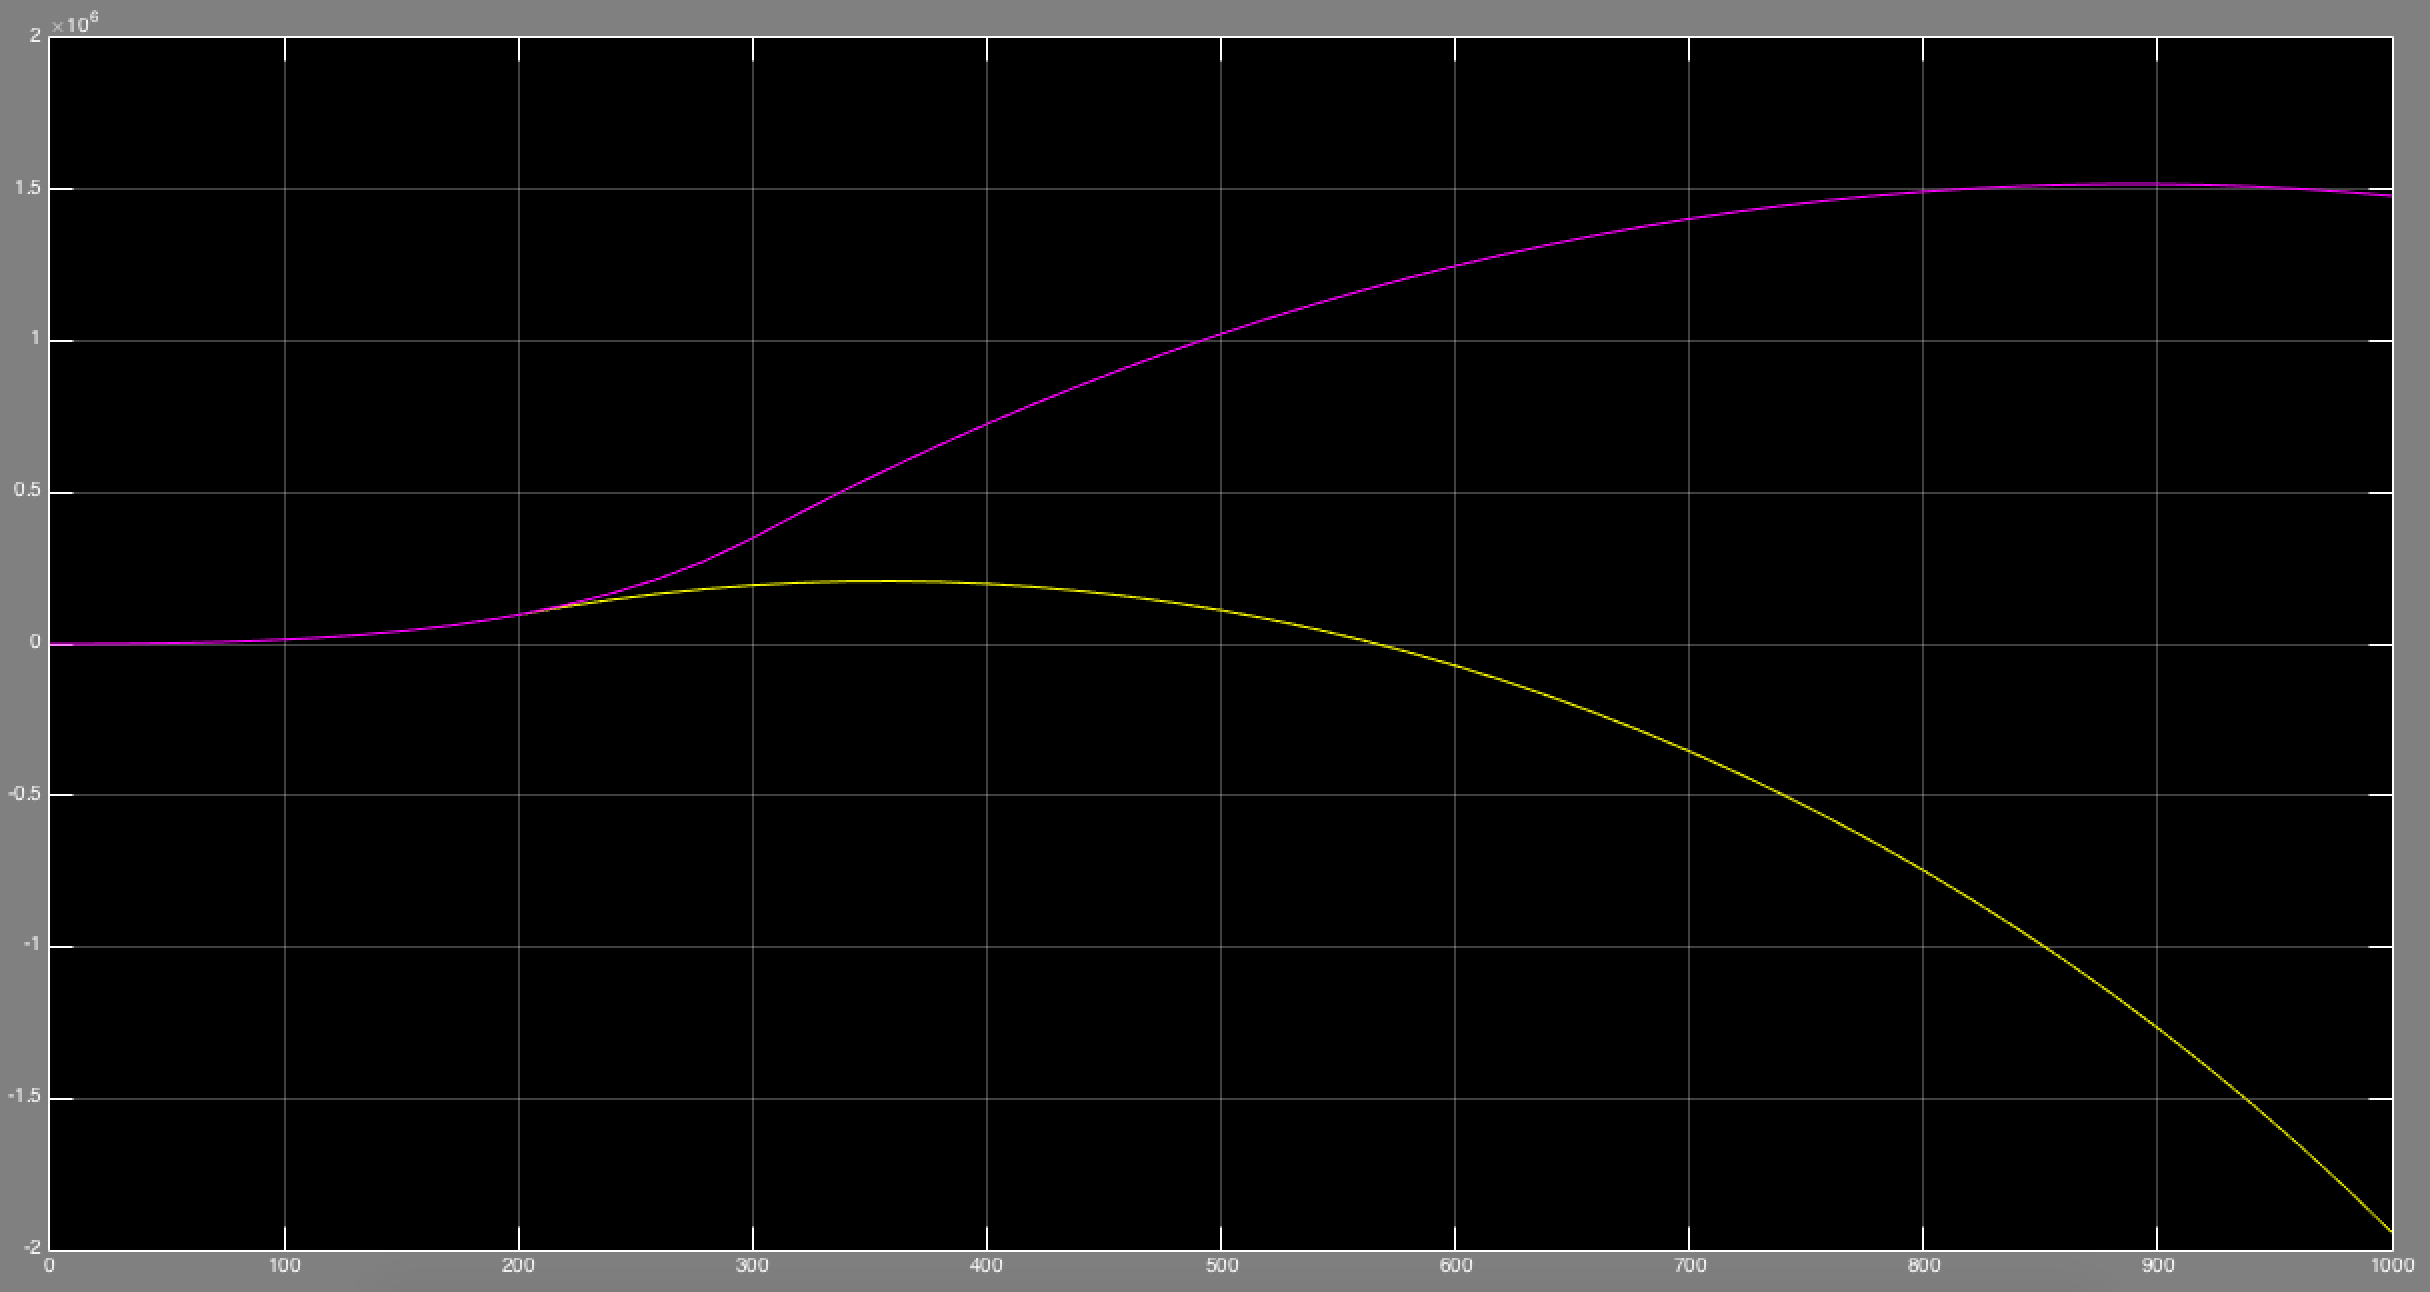
\includegraphics[width=1\textwidth]{../aufgabe1/screens/hoehen.png}
		 	 	 	 		\caption{Höhen}
		 	 	 	 	\end{figure}
\section{Simulation eines schiefen Flippers}
\begin{figure}[H]
	\centering
	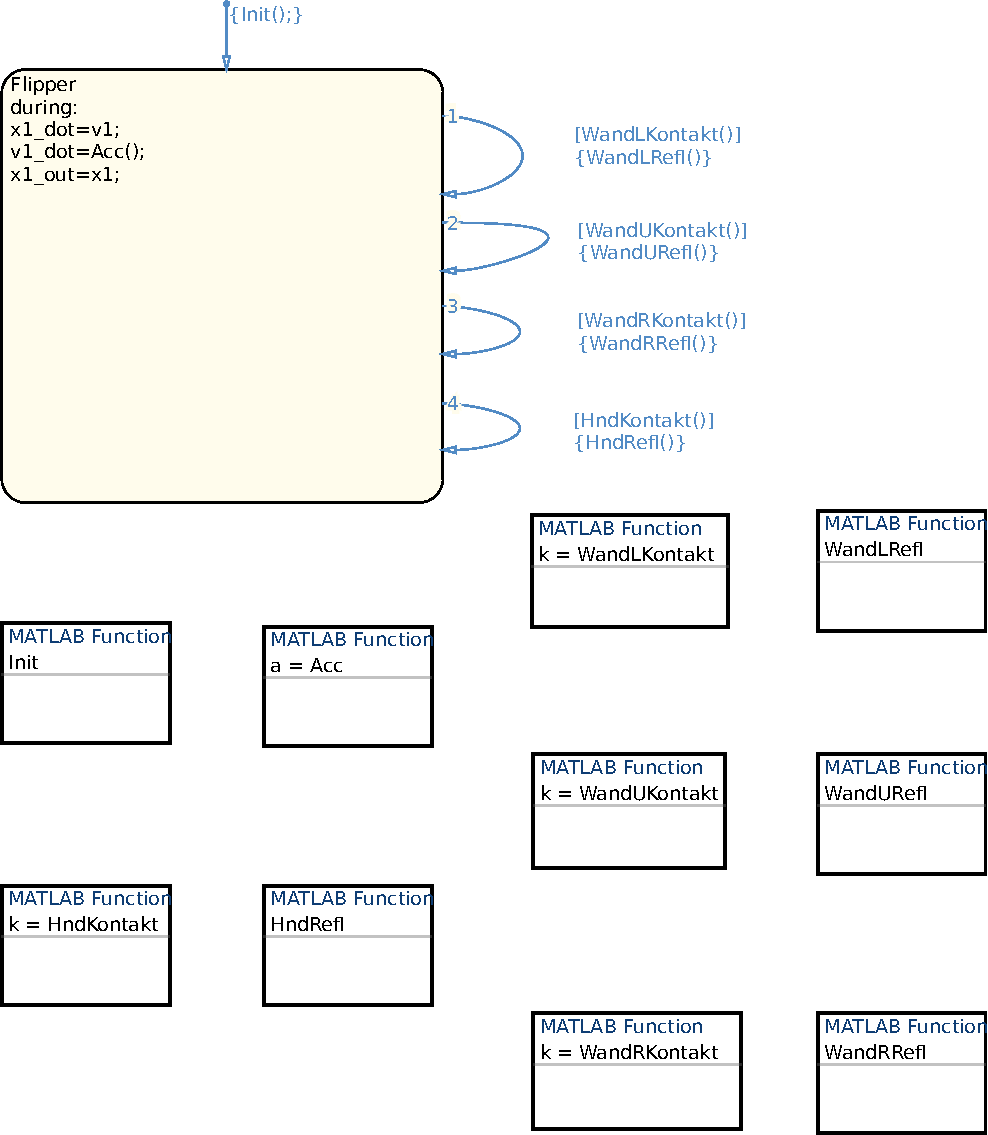
\includegraphics[width=1\textwidth]{../aufgabe2/screens/Flipper}
	 	 	 	 		\caption{Stateflow Flipper}
\end{figure}

\begin{figure}[H]
\begin{lstlisting}
function Init

x1 = [4; 5];
v1 = [0; 0];

p1 = [0; 5];
p2 = [5; 0];
p3 = [9; 0];
p4 = [10; 7];
Hnd = [6; 2.5];

t1 = (p2 - p1)/norm(p2 - p1);
n1 = [-t1(2); t1(1)];

t2 = (p3 - p2)/norm(p3 - p2);
n2 = [-t2(2); t2(1)];

t3 = (p4 - p3)/norm(p4 - p3);
n3 = [-t3(2); t3(1)];
\end{lstlisting}
\caption{Init Funktion}
\end{figure}

\begin{figure}[H]
\begin{lstlisting}
function a = Acc
 
a = [0; -1];
\end{lstlisting}
\caption{Beschleunigung}
\end{figure}

\begin{figure}[H]
\begin{lstlisting}
function k = WandLKontakt
k = false;
if (abs((x1 - p1)' * n1) <= R && (v1' * n1) < 0)
    k = true;
end
\end{lstlisting}
\caption{Wand Links Kontakt}
\end{figure}

\begin{figure}[H]
\begin{lstlisting}
function WandLRefl

vt = v1' * t1;
vn = v1' * n1;

v1 = vt * t1 - vn * n1;
\end{lstlisting}
\caption{Wand Links Reflektion}
\end{figure}

\begin{figure}[H]
\begin{lstlisting}
function k = HndKontakt
k = false;

n = (x1 - Hnd) / norm(x1 - Hnd);
t = [-n(2); n(1)];

if ( norm(Hnd - x1) <= RHnd + R && (v1' * n) < 0)
    k = true;
end
\end{lstlisting}
\caption{Hindernis Kontakt}
\end{figure}

\begin{figure}[H]
\begin{lstlisting}
function HndRefl

n = (Hnd - x1) / norm(Hnd - x1);
t = [n(2); -n(1)];

vt = v1' * t;
vn = v1' * n;

v1 = vt * t - vn * n;
\end{lstlisting}
\caption{Hindernis Reflektion}
\end{figure}

\end{document}
